\chapter{Ingeniería de Software Ágil}

\section{Proceso de desarrollo}

Hacer agilidad no nos asegura calidad. Para ello primero hay que asegurarse de hacer ingeniería de software además de agilidad. Hay diferentes procesos de ingeniería y podemos tomar el siguiente: descubrimiento y definición de requerimientos (Discovery \& Requirements), análisis y diseño (Analysis \& Design), implementación y pruebas (Implementation \& Testing), integración y pruebas (Integration \& Testing), despliegue (Delivery) y monitoreo (Monitoring). Hay que considerar que el proceso de Ingeniería de Software sobre una pieza de Software (feature o historia), si bien es secuencial, tiene las fases que se solapan. 

\begin{figure}[h]
  \centering
  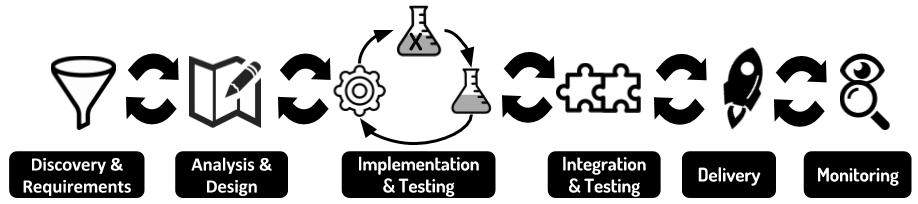
\includegraphics[width=0.99\textwidth]{PhasesOfSoftwareEngineering}
  \caption{Ciclo de ingeniería de Software}
  \centering
  \label{fig:PhasesOfSoftwareEngineering} %\ref{fig:PhasesOfSoftwareEngineering}
\end{figure}

Correr este proceso bajo un marco ágil como Scrum, con prácticas ágiles es lo que podemos llamar Ingeniería de Software Ágil (Agile Software Engineering). Además es conveniente introducir la idea de prácticas continuas, es decir refinamiento continuo (análisis y diseño con trabajo UX continuo), testing continuo (continuous testing), integración continua (continuous integration), despliegue o entrega continua (continuous deployment \& continuous delivery) y monitoreo continuo (continuous monitoring). 
Dicho esto, tenemos que tener en cuenta cómo unir y ajustar el proceso de Ingeniería de Software con el marco de trabajo Scrum. En este sentido es que se plantea ejecutar las fases del proceso de ingeniería, sobre historias de usuario, dentro del tren de sprints. En un equipo extremadamente autónomo y ágil, todas las fases se pueden desarrollar bajo el tren de sprints de Scrum.

\begin{figure}[h]
  \centering
  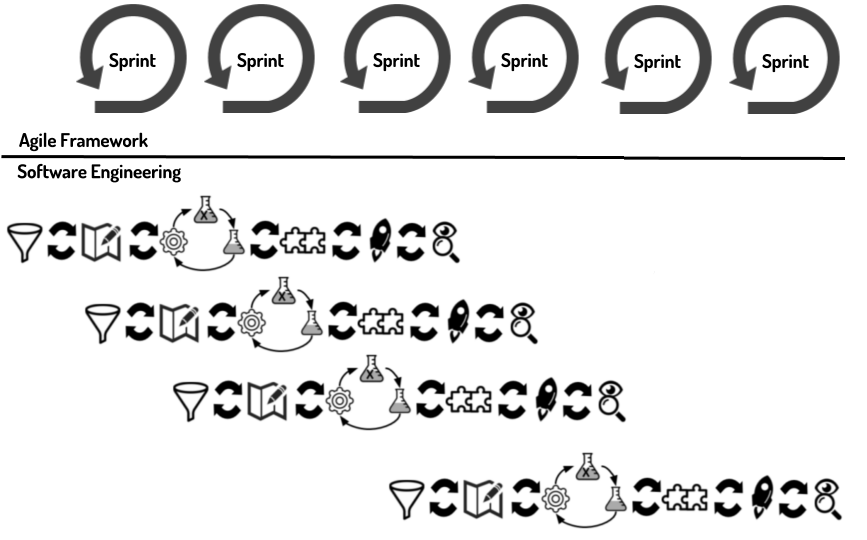
\includegraphics[width=0.99\textwidth]{AgileSoftwareEngineering}
  \caption{Ingeniería de Software Ágil}
  \centering
  \label{fig:AgileSoftwareEngineering} %\ref{fig:AgileSoftwareEngineering}
\end{figure}

De este modo, se integra el testing en fases más tempranas del desarrollo, por lo que QA no retrasa al equipo de desarrollo, porque QA está dentro del equipo y se trabaja con testing continuo. Los mismo sucede con UX y Operaciones.

\section{Prácticas técnicas}

Como ya he mencionado, es deseable que el SM vele por la excelencia técnica de su equipo y del proceso de desarrollo buscando lograr un flujo limpio. Claro que la responsabilidad es del equipo y tanto un líder técnico como el SM, puede liderar o guiar el proceso de mejora continua del flujo. Teniendo en cuenta las fases de desarrollo de los ítems de trabajo como historias, podemos tener dos aspectos en consideración para analizar el estado de nuestro procesos de desarrollo en cuanto a excelencia técnica. Por un lado, el aspecto de prácticas técnicas considerando la información, proceso, métodos, técnicas y organización (aquí se tiene en cuenta XP entre otras cosas). Por otro lado el aspecto tecnológico considerando las herramientas empleadas que cubren estas prácticas técnicas. Por ejemplo a continuación muestro un esquema de flujo y sus prácticas técnicas relacionadas.

\begin{figure}[h]
  \centering
  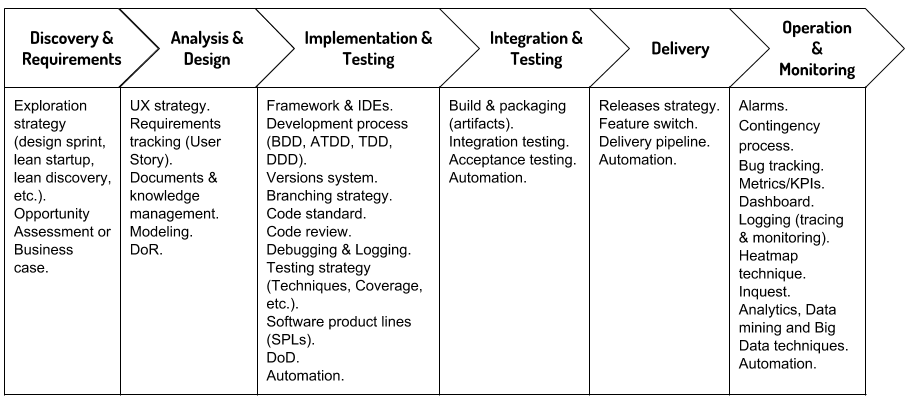
\includegraphics[width=0.99\textwidth]{TechnicalPractices}
  \caption{Flujo de prácticas técnicas}
  \centering
  \label{fig:TechnicalPractices} %\ref{fig:TechnicalPractices}
\end{figure}

Se puede hacer un esquema de flujo semejante con los aspecto tecnológico, herramientas, correspondientes a cada fase.

\section{En síntesis}

Hacer ingeniería de software ágil es desarrollar software de valor, de modo iterativo e incremental, con un producto o servicio que evoluciona, donde los requisitos y soluciones evolucionan con el tiempo, haciendo entregas frecuentes de calidad y valor, trabajando con equipos auto-organizados y multidisciplinarios que mejoran, inmersos en un proceso compartido de toma de decisiones interactiva y dinámica. Y, lo más importante, es considerar que la ingeniería es, además de una práctica científica, una práctica humana. Construir software se trata de relaciones humanas en un sistema social. Por eso, hay que construir relaciones humanas de valor, que habiliten la entrega continua de valor.
